% !TeX spellcheck = en_US
\documentclass[11pt, a4paper]{article}
\usepackage[utf8]{inputenc}

\usepackage{latexsym}
\usepackage{float}
\usepackage[utf8]{inputenc}
\usepackage[english]{babel}
\usepackage{microtype}
\usepackage[hyphens]{url}
\usepackage{hyperref}
\usepackage{graphicx}
\usepackage[nonumberlist,acronym]{glossaries}
\usepackage{makeidx}
\usepackage{datetime}
\usepackage{multicol}
\usepackage{setspace}
\usepackage{pdflscape}
\usepackage{pgffor}
\usepackage{enumerate}
\usepackage{booktabs}
\usepackage{tabularx}
\usepackage{braket}
\usepackage{listings}
\usepackage{color}
\usepackage{amsmath}
\usepackage{amssymb}
\usepackage[table,xcdraw]{xcolor}
\usepackage{graphicx}
\usepackage{listings}
\usepackage{hyperref}
\usepackage{vmargin}
\usepackage{wrapfig}
\usepackage{subfiles}
\usepackage{float}
\usepackage{amsmath}
\usepackage{amssymb}
\usepackage{tikz-cd}
\usepackage{multirow}
\usepackage{pgffor}
\usepackage{enumitem}
\usepackage{iflang}
\usepackage{varioref}
\usepackage{hyperref}
\usepackage{cleveref}
\usepackage{caption}
\usepackage{subcaption}
\usepackage{tikz}
\usepackage{enumitem}
\usepackage{xpatch}
\usepackage{refcount}
\usepackage{color}
\usepackage{pdfpages}
\usepackage{array}
\usepackage{eurosym}


%%%%%%%%%%%%%%%%%%%%%%%%%%%%%%%%%%%%%%%
%%%%%%%%%%%% UTIL COMMANDS %%%%%%%%%%%%  

\setcounter{secnumdepth}{4}
\newcommand{\nc}{\newcommand}
\nc{\supindex}{\textsuperscript}
\renewcommand{\baselinestretch}{1.5}
\nc{\myparagraph}[1]{\paragraph{#1}\mbox{}\\}

%%%%%%%%%%%%%%%%%%%%%%%%%%%%%%%%%%%%%%%
%%%%%%%%%%%%% CONFIG FILE %%%%%%%%%%%%%

\nc{\mytitle}{Economic Viability}
\nc{\mysubtitle}{Bayesian Inference}
\nc{\authors}{\textit{Oriol Alàs Cercós}}
\nc{\datetime}{25\supindex{th} of May, 2022}
\nc{\assignatura}{Technological Business Management and Entrepreneurship}
\nc{\professorat}{Josep Escribà Garriga}

% Per separar professors, utilitzar ','
% 	Ex: Maria, Joan, Pere

%%%%%%%%%%%%%%%%%%%%%%%%%%%%%%%%%%%%%%%
%%%%%%%%%%%%%  LANGUAGE   %%%%%%%%%%%%%

\newcommand{\tr}{\IfLanguageName{english}}

%%%%%%%%%%%%%%%%%%%%%%%%%%%%%%%%%%%%%%%
%%%%%%%%%%%%%%%%% MATH %%%%%%%%%%%%%%%%

\nc{\prob}[1]{P({#1})}
\nc{\probl}[2]{P({#1}|{#2})}

%%%%%%%%%%%%%%%%%%%%%%%%%%%%%%%%%%%%%%%
%%%%%%%%%%%%% FUNCTIONS %%%%%%%%%%%%

\nc{\numitems}[1]{\getrefnumber{#1}}
\newcounter{itemcntr}
\AtBeginEnvironment{itemize}{%
	\setcounter{itemcntr}{0}%
	\xapptocmd{\item}{\refstepcounter{itemcntr}}{}{}%
}

%%%%%%%%%%%%%%%%%%%%%%%%%%%%%%%%%%%%%%%
%%%%%%%%%%%%% RADIO BUTTON %%%%%%%%%%%%

\makeatletter
\newcommand*{\radiobutton}{%
	\@ifstar{\@radiobutton0}{\@radiobutton1}%
}
\newcommand*{\@radiobutton}[1]{%
	\begin{tikzpicture}
		\pgfmathsetlengthmacro\radius{height("X")/2}
		\draw[radius=\radius] circle;
		\ifcase#1 \fill[radius=.6*\radius] circle;\fi
	\end{tikzpicture}%
}
\makeatother


%%%%%%%%%%%%%%%%%%%%%%%%%%%%%%%%%%%%%%%
%%%%%%%%%%%%%  %%%%%%%%%%%%


\newcolumntype{S}{>{\centering\arraybackslash}m{1.5em}}

\renewcommand{\tabularxcolumn}[1]{m{#1}} % redefine 'X' to use 'm'
\newcommand{ \titem}[1]{\item \textbf{#1}\quad}

\newcommand{\costVar}[4]{In that moment, we want to earn $\frac{#1\text{€}}{1 h}$, therefore the human resource cost will be: \[#2 \cdot \frac{#3h}{1 day} \cdot \frac{#1\text{€}}{1 h} = #4 \text{€}\] }

\nc{\numbers}[1]{
	\begin{tabularx}{#1\textwidth}{|S|S|S|S|S|}
		\hline 1 & 2 & 3 & 4& 5 \\\hline
	\end{tabularx}
}

\nc{\optionsofcol}{
	\multicolumn{3}{c}
	{%
		\numbers{0.338}
	}
}

\nc{\options}{\multicolumn{2}{c}
	{%
		\numbers{0.338}
}}

\newcommand{\costHR}[4]{\[Cost_{\text{HR}} = #1 \frac{\text{€}}{h} \cdot \frac{#2 \, \, \text{hours}}{\text{day}} \cdot #3 \, \, \text{days} = #4 \, \, \text{€} \]}

\newcolumntype{P}[1]{>{\centering\arraybackslash}p{#1}}

\setpapersize{A4}

\author{Oriol Alàs Cercós}
\date{29 d'Abril del 2019}

\makeglossaries
\newacronym{rs}{RS}{Remote Sensing}
\newacronym{sar}{SAR}{Synthetic Aperture Radar}
\newacronym{cnn}{CNN}{Convolutional Neural Network}
\newacronym{gan}{GAN}{Generative Adversarial Network}
\newacronym{mcgan}{McGAN}{Multi-spectral Conditional Generative Adversarial Network}
\newacronym{nir}{NIR}{Near Infra Red}
\newacronym{nlp}{NLP}{Natural Language Processing}
\def\contentsname{Índex}
\begin{document}
	
	\definecolor{gray}{rgb}{0.4,0.4,0.4}
	\definecolor{darkblue}{rgb}{0.0,0.0,0.6}
	\definecolor{cyan}{rgb}{0.0,0.6,0.6}
	\lstset{
		basicstyle=\ttfamily,
		columns=fullflexible,
		showstringspaces=false,
		commentstyle=\color{gray}\upshape
	}
	
	\lstdefinelanguage{XML}
	{
		morestring=[b]",
		morestring=[s]{>}{<},
		morecomment=[s]{<?}{?>},
		stringstyle=\color{black},
		identifierstyle=\color{darkblue},
		keywordstyle=\color{cyan},
		morekeywords={xmlns,version,type}% list your attributes here
	}
	
	\begin{titlepage}
		\begin{figure}[htb]
			\begin{center}
				
				\includegraphics[width=5cm]{imgs/udl.png}\\
				
				
				\medskip
				\begin{center}
					
					\huge\textbf{\mytitle}\\
					\bigskip
					\normalsize{\tr{Made by}{Realitzat per:}}
					\\
					\large\textit{\authors}
					\\
					\setlength{\parskip}{1em}
					\normalsize{\tr{Delivery}{Data de lliurament:}}
					\\
					\large{\datetime}
				\end{center}
				
				\vspace*{\stretch{2.0}}
			\end{center}
		\end{figure}
		\begin{flushright}
			Universitat de Lleida
			\\
			Escola Politècnica Superior
			\\
			Màster en Enginyeria Informàtica
			\\
			\assignatura
			\\
			\medskip
			\textbf{\tr{Professorate:}{Tutor:}}
			\\
			\foreach \n in \professorat{\n\\}
		\end{flushright}
		\thispagestyle{empty} 
	\end{titlepage}
	\pagenumbering{roman}
	\tableofcontents
	\listoffigures
	\newpage
	\pagenumbering{arabic}
	\printglossary[type=\acronymtype]
	\newpage
	\section{Introduction} 
	\gls{rs} imagery is critical to perform challenges such climate change or natural resources management, including zone monitoring for reforestation, disaster mitigation and land surface change detection.  % canvi de terrenys, natural resources management, climate change, zone monitoring for reforestation, climate change, disaster mitigation 
	Nevertheless, on average 55\% of the Earth's land surfaces is covered by clouds, being then a significant impediment to carry out a broad range of applications. Satellite imagery plagued by films of clouds that obstructs the scene implies a great loss of information or causing effects such as blurring, which mitigates the power of \gls{rs}. Hence, \gls{rs} applications definitely needs a generic technique to detect and remove the cloudy region with an in-painting of the underlying scene.
	\\
	\\
	\begin{itemize}
		\item Generic end-to-end model that can be retrained for specifically ROI by running supplementary iterations but general enough to be great in all geographical locations.
		\item Free.
	\end{itemize}
	\subsection{Sentinel2}
	Sentinel2 images are provided by two satellites, Sentinel 2A and Sentinel 2B, which orbit each other with a 180º phase shift. The acquisition of the images is 10 days per satellite or 5 days altogether. Therefore, a new updated image of a specific area is available in periods of time not exceeding five days. This makes Sentinel-2 data an excellent choice for studying environmental challenges. Sentinel-2 data is multi-spectral with 13 bands in the visible, near-infrared, and short-wave infrared spectrum. These bands come in a different spatial resolution ranging from 10m to 60m, so the images can be classified as medium-high resolution.
	\subsection{Related work and state-of-the-art}
%	Questions:
%	\begin{itemize}
%		\item Cloud detection / Cloud removal
%		\item Which dataset uses?
%		\begin{itemize}
%			\item Bandwidths
%			\item Sparse ROI? How many? Multi-source?
%			\item Pair dataset?
%			\item Multi-Temporal?
%		\end{itemize}
%		\item Model
%		\begin{itemize}
%			\item Fully CNN?
%			\item Residual?
%			\item Needs pair dataset?
%			\item Has a skip connection? Structure of U-Net?
%			\item GAN?
%		\end{itemize}
%		\item Metrics
%	\end{itemize}
	Deep learning have been a popular and efficient technique to solve challenges from satellite imagery. Specifically, \gls{cnn} have been the main architecture of neural networks to provide a solution from image-based problems. 
	\\
	\\
	In \cite{LANARAS2018305}, they create a deep learning approach to Sentinel-2 super-resolution. Their hypothesis was the existence of a complex mixture of correlations across many spectral bands over a large spatial context. Hence, the input of the model is a concatenation of the high-level resolution bands with the low-level resolution bandwidths upsampled to 10m by simple bi-linear interpolations. The model itself is a clear reference of residual networks \cite{he2016deep}. Furthermore, as in ResNet architectures, it uses skip connections to reduce the average effective path length through the network, alleviate the vanishing gradient problem and greatly accelerates the learning.
	\begin{figure}[H]
		\centering
		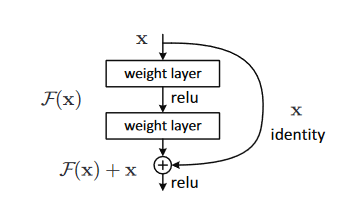
\includegraphics[width=6cm]{imgs/relatedwork/residualblock.png}
		\caption{Residual learning: a building block.}
	\end{figure}
	Similarly, in \cite{Meraner2020}, a residual network is used with the same skip connections mechanism to bring a solution to cloud removal challenge. It also uses
	\gls{sar} 
	optical data, which represents an important complementary source to help the model to make greater results. However, \gls{sar} images are affected by a particular type of noise called speckle, which can difficult network's learning. Moreover, the model depends on one more source to remove the clouds, as \gls{sar} images cannot be downloaded in Sentinel-2. Regarding the design of the neural network, 
	DSen2-CR is a fully convolutional network, so it can accept input images of any spatial dimensions (\textit{m}), as it can be seen in \ref{fig:dsen2-cr}.
	The  output of DSen2-CR is a 13-channel layer, representing the thirteen bands from Sentinel2.  
	\begin{figure}[H]
		\centering
		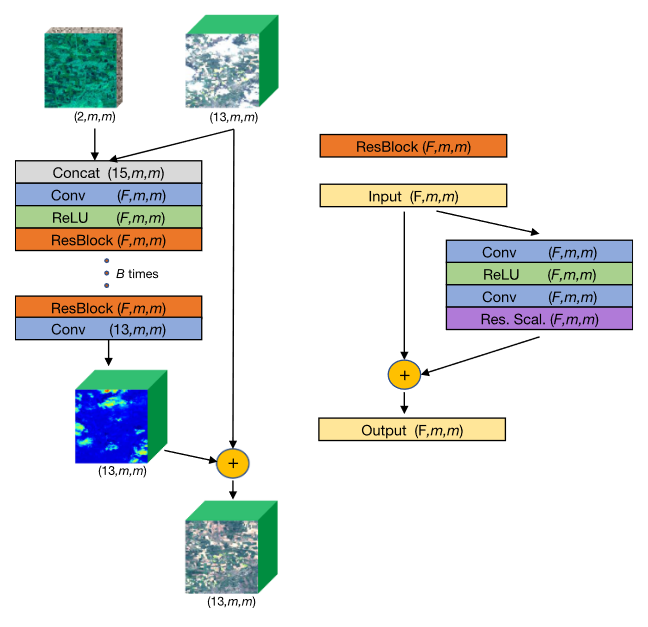
\includegraphics[width=10cm]{imgs/relatedwork/sar.png}
		\caption{DSen2-CR model diagram.}
		\label{fig:dsen2-cr}
	\end{figure}
	Improvements have been found using \gls{gan} \cite{goodfellow2014generative}, which is a model architecture that belongs to the set of generative models. \gls{gan} is an unsupervised model made up of two neural networks. The idea is based on a game theoretic scenario in which the generator network must compete against an adversary. While the generator network produces samples, the aim of the discriminator is to distinguish between the real samples and the drawn by the generator. 
	\\
	\\
	During training, both networks constantly try to outsmart each
	other, in a zero-sum game. At some point of the training, the game may end up in a state that
	game theorists call a Nash equilibrium, when no player would be better off changing their own strategy, assuming the other players do not change theirs. \gls{gan}s can only reach one possible Nash equilibrum, which is when the generator produces so realistic images that the discriminator is forced to guess by 50 \% probability that the image is real or not. Nevertheless, the training process not always can converge to Nash equilibrium. There are several factors that make the training hard to reach the desired state. For instance, there is a possibility that the discriminator always outsmarts the generator so that it can clearly distinguish between fake and real images. As it never fails, the generator is stuck trying to produce better images as it cannot learn from the errors of the discriminator. Possible solutions can be carried out such as making the discriminator less powerful, decreasing the learning rate or adding noise to the discriminator target. Another big obstacle is when the generator becomes less diverse, and it learns only to perfectly generate realistic images of a single class, so it forgets about the others. This is  called mode collapse. At some point, the discriminator can learn how to beat the generator, but then the latter is forced to do the same but in another class, cycling between classes never becoming good at any of them. A popular technique to avoid is experience replay, which consists in storing synthetic images at each iteration in a replay buffer. There is a lot of literature of obstacles and solutions to improve \gls{gan} training and it is still very active, as it is in its applications too.
	\\
	\\
	Regarding cloud removal, in \cite{8014931}, Enomoto %TODO change name
	proposed a  \gls{mcgan} trained using RGB and \gls{nir} cloud-free bands as input and synthetic RBG cloudy images as target. It is true that short wave bands are unaffected by cloud cover and using \gls{nir} images to guide to uncover the clouds of satellite imagery is great since \gls{nir} bands posses have higher penetration through fog than visible light bands. Nevertheless, synthetizing the target might not be realistic enough to feasibly deploy the model in real-state. \cite{sarukkai2019cloud} proposed two models. The first, similar to \cite{8014931}, is trained by a paired dataset of single-images in the input as well as in the output although cloudy imagery is not synthesized. The second is a spatio-temporal \gls{gan} trained by pairing clear images with several corresponding cloudy ones from diverse points in time. 
	\\
	\\
	Cloud-GAN \cite{8519033} is a cyclic \gls{gan} which uses two generators and two discriminators. Cyclic \gls{gan}s can create new samples of output data, but also transforming the desired data to samples of input data. In essence, they learn to transform data from the two sources by the two generators respectively. In this case, the generator $G_A$ is generating cloud-free images from cloudy images while the generator $G_B$ is turning the cloud-free images into cloudy. Hence, there is no need to train the model by paired cloudy-cloud-free imagery\footnote{Paired cloudy-cloud-free dataset means to have images from the same zone with and without clouds in order to compare the output data with the cloud-free data.}.
	\\
	\\
	Training a CycleGAN using only the two network losses does not guarantee that cycle consistency is held. Thus, an additional cycle consistency loss is used to enforce this property. This loss is defined as the absolute value difference (L1 norm) between an input value x and it's forward-cycle prediction F(G(x)), as well as the input values y and their forward-cycle prediction G(F(y)). The higher the difference, the more distant the predictions are from the original inputs. Ideally, our network would minimize this loss.
	\\
	\\
	Although \gls{cnn} have worked very well for cloud removal, latest and disruptive state-of-the-art deep learning attention-based architectures \cite{VaswaniSPUJGKP17} uncover new paths to achieve remarkable improvements and results. It has been demonstrated that transformers can excellently overcome challenges such \gls{nlp} \cite{brown2020language} 
	, Text-To-Image Generation \cite{pmlr-v139-ramesh21a}  or Image Completion \cite{pmlr-v119-chen20s} with large datasets, great model size and enough compute. Recent contributions have been demonstrated that 
	\section{Data}
	\subsection{Academic Datasets}
	\section{Model architecture}
	
	\section{Experiments \& results}
	\section{Conclusions}
	\section{Bibliography}

	\bibliography{bibliography}
	\bibliographystyle{unsrt}
\end{document}